\begin{question}[section=11,name={Drehkreuzantenne 2},difficulty=,quantity=6,type=thr,tags={20130314,20060816}]
	Skizieren Sie eine Drehkreuzantenne inklusive der Speiseleitung!
	\\ \textbf{Hinweis:}\\
	Skript Seite 112
\end{question}
\begin{solution}
	\begin{figure}[H]
		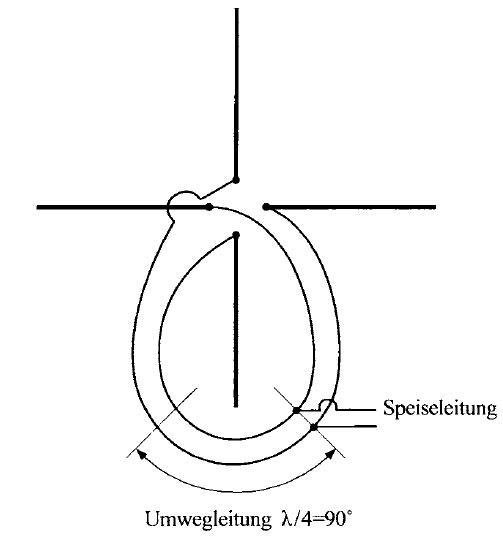
\includegraphics[width=14cm]{./opn/exm/thr/chp/11/3/bild.jpeg}
	\end{figure}
	Zwei Dipole um 90\degree gegeneinander verdreht. Die Speiseleitung eines Dipols ist um $\lambda/4$ länger. Dadurch ergibt sich eine Phasenverschiebung um 90\degree, und eine Drehpolarisation.
\end{solution}
